\section{Results}
\subsection{Minikube results}
After running the commands in Listings~\ref{lst:minikube-cluster}, the Minikube creates a three-node cluster with two worker nodes and one control plane node.
This is shown in Figure~\ref{fig:minikube-cluster}.

\begin{figure}[htbp]
  \centering
  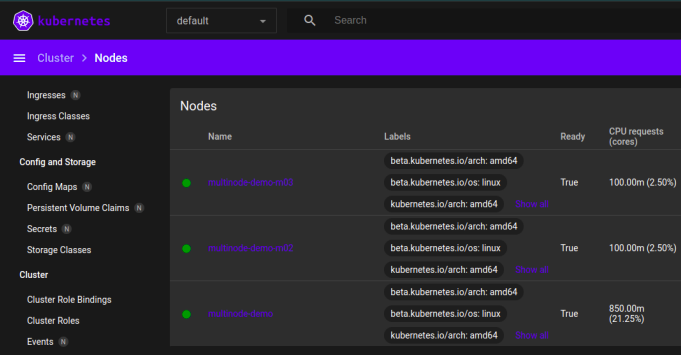
\includegraphics[width=0.45\textwidth]{figures/nodes.png}
  \caption{Minikube cluster with three nodes.}
  \label{fig:minikube-cluster}
\end{figure}

After running the commands in Listings~\ref{lst:kubectl_php_apache}, the PHP Apache server is deployed on the Minikube cluster.
The dashboard shows the deployment and service created, as shown in Figure~\ref{fig:deployments} and Figure~\ref{fig:services}, respectively.

\begin{figure}[htbp]
  \centering
  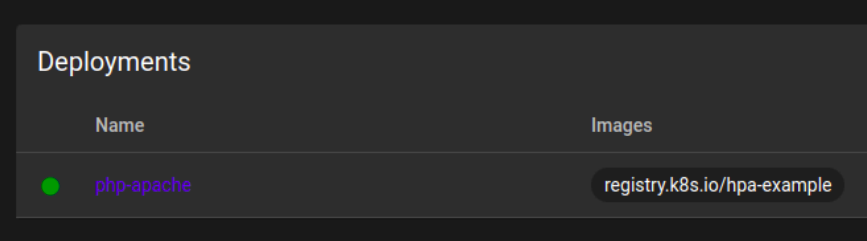
\includegraphics[width=0.45\textwidth]{figures/deployments.png}
  \caption{PHP Apache server deployment.}
  \label{fig:deployments}
\end{figure}

\begin{figure}[htbp]
  \centering
  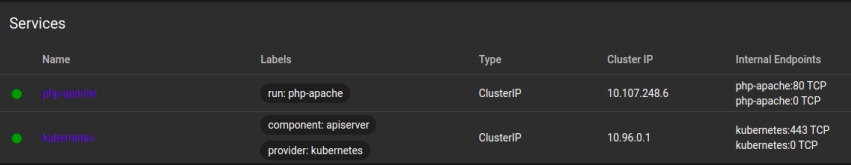
\includegraphics[width=0.45\textwidth]{figures/services.png}
  \caption{PHP Apache server service.}
  \label{fig:services}
\end{figure}

Then, the Horizontal Pod Autoscaler (HPA) is configured to scale the PHP Apache server deployment based on CPU usage.


\subsection{AWS EKS results}

After the execution of the commands to test the autoscaler, as outlined in Listing~\ref{lst:autoscaler-test}, The output of this command is presented in Figure~\ref{fig:metrics}.

\begin{figure}[htbp]
  \centering
  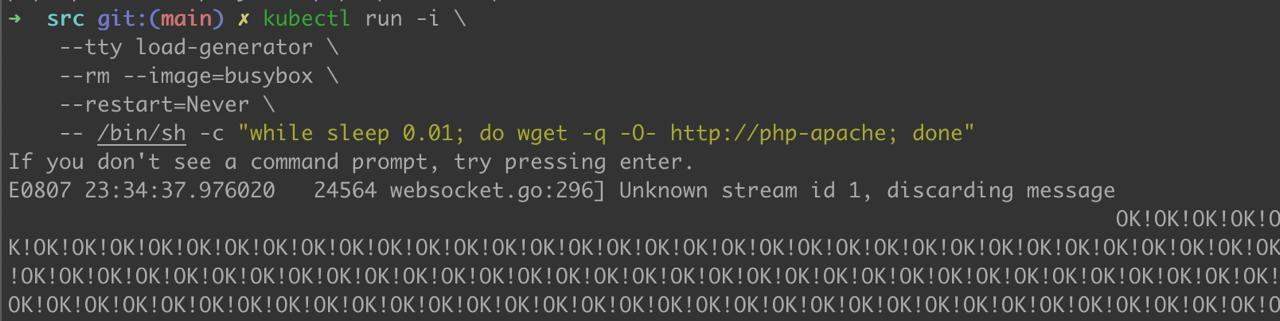
\includegraphics[width=0.45\textwidth]{figures/test-autoscaler.jpeg}
  \caption{Test autoscaler on EKS.}
  \label{fig:test-autoscaler}
\end{figure}

Next, we allowed approximately 2.5 minutes to elapse before proceeding with the command that displays the number of replicas managed by the autoscaler, as shown in Listing~\ref{lst:pods-number}. The output of this command is presented in Figure~\ref{fig:metrics}, where it is evident that nine replicas of the server were generated in response to the load induced by the test command.

\begin{figure}[htbp]
  \centering
  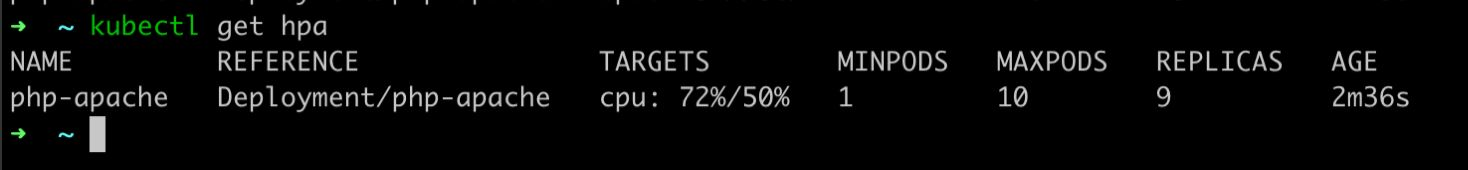
\includegraphics[width=0.45\textwidth]{figures/metrics.jpeg}
  \caption{PHP Apache server metrics.}
  \label{fig:metrics}
\end{figure}